% -*- latex -*-
%%%%%%%%%%%%%%%%%%%%%%%%%%%%%%%%%%%%%%%%%%%%%%%%%%%%%%%%%%%%%%%%
%%%%%%%%%%%%%%%%%%%%%%%%%%%%%%%%%%%%%%%%%%%%%%%%%%%%%%%%%%%%%%%%
%%%%
%%%% This text file is part of the source of 
%%%% `Parallel Programming in MPI and OpenMP'
%%%% by Victor Eijkhout, copyright 2012-9
%%%%
%%%% petsc-objects.tex : petsc tangible-ish objects
%%%%
%%%%%%%%%%%%%%%%%%%%%%%%%%%%%%%%%%%%%%%%%%%%%%%%%%%%%%%%%%%%%%%%
%%%%%%%%%%%%%%%%%%%%%%%%%%%%%%%%%%%%%%%%%%%%%%%%%%%%%%%%%%%%%%%%

\Level 0 {Distributed objects}

PETSc is based on the \ac{SPMD} model, and all its objects act like
they exist in parallel, spread out over all the processes.  Therefore,
prior to discussing specific objects in detail, we briefly discuss how
PETSc treats distributed objects.

For a matrix or vector you need to specify the size. This can be done two ways:
\begin{itemize}
\item you specify the global size and PETSc distributes the object over the processes, or
\item you specify on each process the local size
\end{itemize}
If you specify both the global size and the local sizes, PETSc will check for consistency.

For example, if you have a vector of $N$ components, or a matrix of $N$
rows, and you have $P$ processes, each process will receive $N/P$
components or rows if $P$ divides evenly in~$N$. If $P$ does not divide
evenly, the excess is spread over the processes.

The way the distribution is done is by contiguous blocks: with 10
processes and 1000 components in a vector, process 0 gets the range
$0\cdots99$, process 1 gets $1\cdots199$, et cetera. This simple scheme suffices for
many cases, but PETSc has facilities for more sophisticated load
balancing.

Once an object has been created and distributed, you do not need to
remember the size or the distribution yourself: you can query these
with calls such as \lstinline{VecGetSize},
\lstinline{VecGetLocalSize}, and \lstinline{VecGetOwnershipRange}.

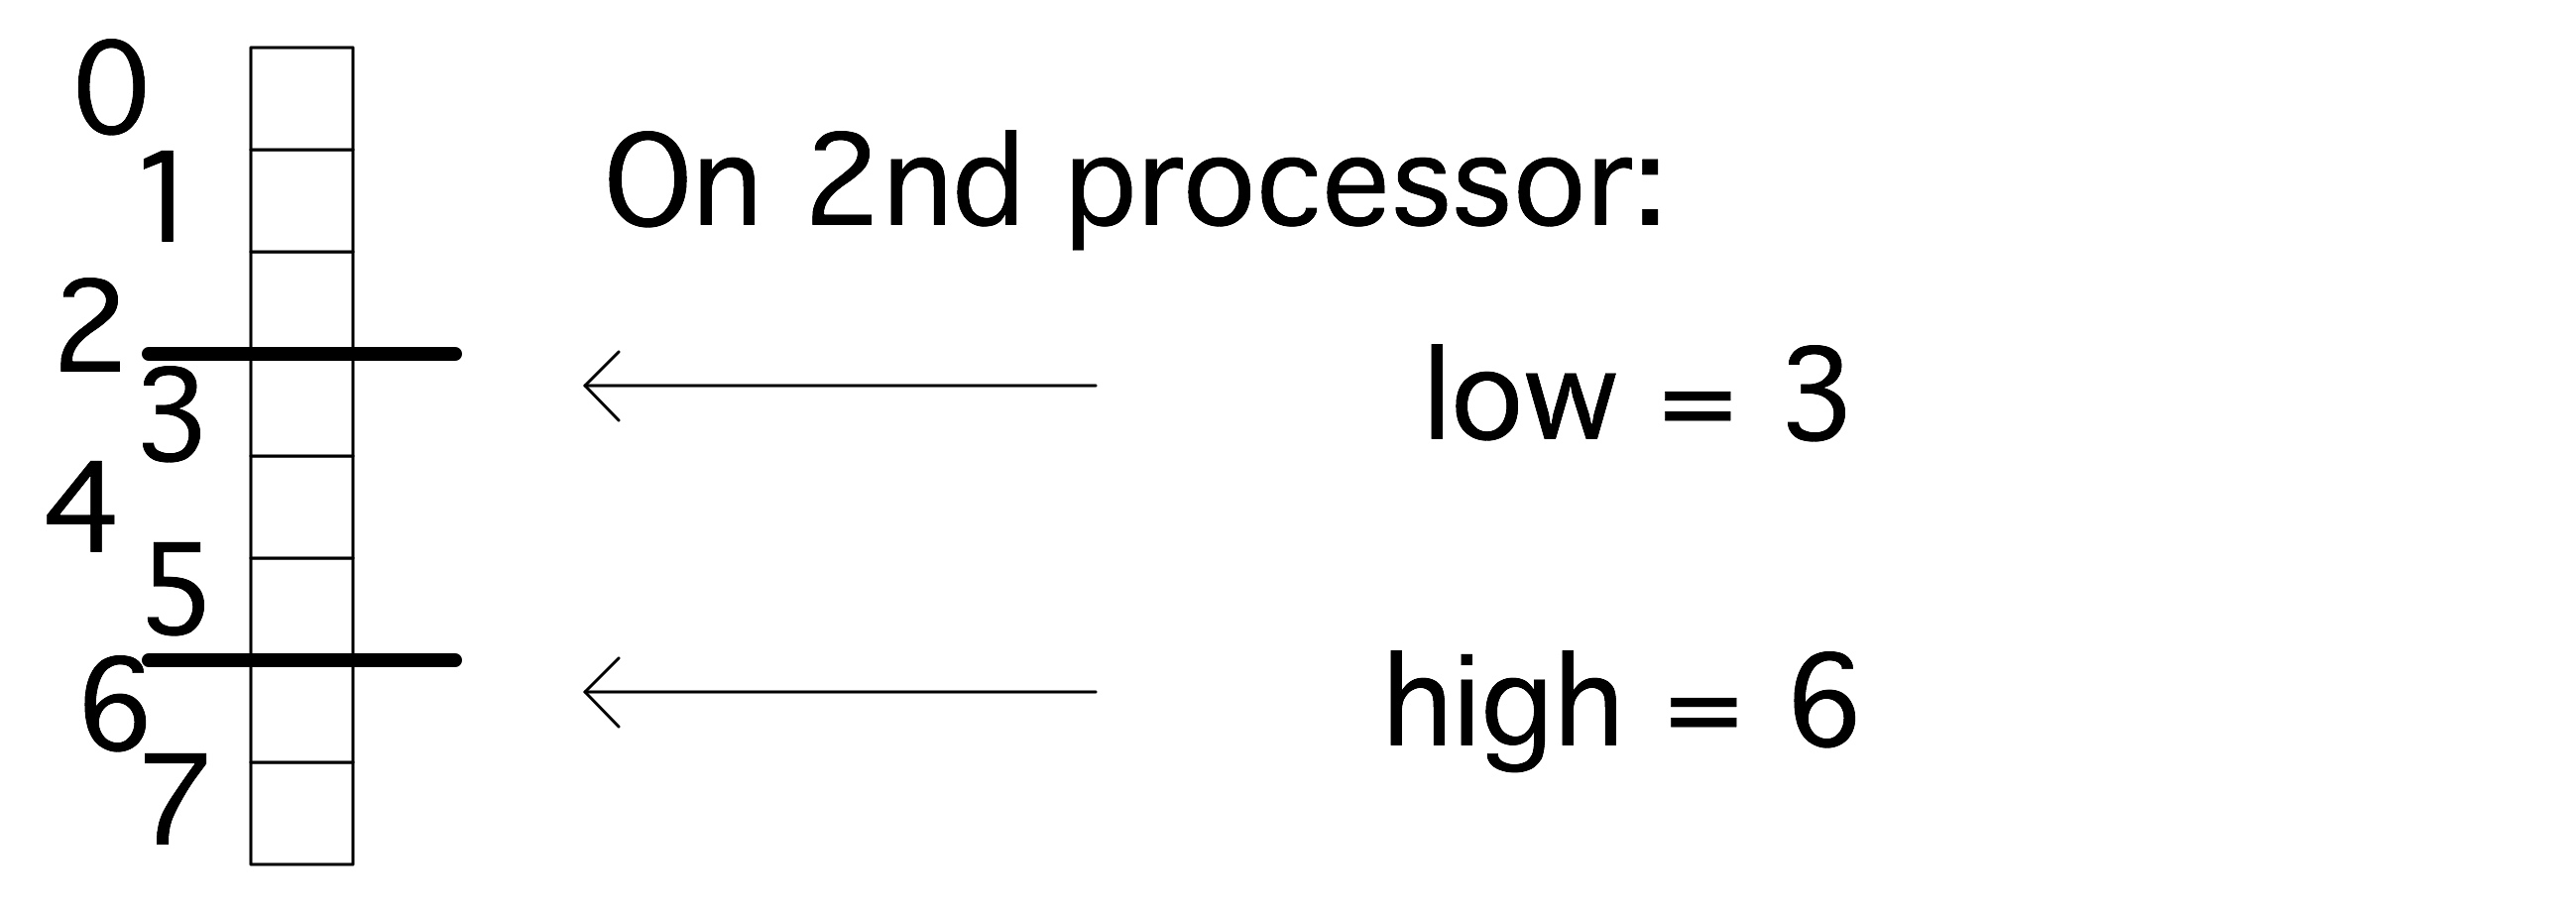
\includegraphics[scale=.1]{veclayout}

The
corresponding matrix routines \lstinline{MatGetSize},
\lstinline{MatGetLocalSize} give both information for the
distributions in $i$ and~$j$ direction, which can be
independent. Since a matrix is distributed by rows,
\lstinline{MatGetOwnershipRange} only gives a row range.

These conversions between local and global size can also be done
explicitly, using the \indexpetscref{PetscSplitOwnership} routine.
This routine takes two parameter, for the local and global size, and
whichever one is initialized to \indexpetscshow{PETSC_DECIDE} gets
computed from the other.

\Level 0 {Scalars}
\label{sec:petsc-scalar}

Unlike programming languages that explicitly distinguish between
single and double precision numbers, PETSc has only a single scalar
type: \indexpetscdef{PetscScalar}. The precision of this is determined
at installation time. In fact, a \lstinline{PetscScalar} can even be a
complex number if the installation specified that the scalar type is
complex.

Even in applications that use complex numbers there can be quantities
that are real: for instance, the norm of a complex vector is a real
number. For that reason, PETSc also has the type
\indexpetscdef{PetscReal}.

Integers in PETSc are likewise of a size determined at installation
time: \indexpetscdef{PetscInt} can be 32 or 64 bits. Furthermore,
there is a \indexpetscdef{PetscErrorCode} type for catching the return
code of PETSc routines.

\Level 0 {Vectors}

Vectors are objects with a linear index. The elements of a vector are
floating point numbers or complex numbers (see
section~\ref{sec:petsc-scalar}), but not integers: for that see
section~\ref{sec:petsc-is}.

\Level 1 {Vector construction}

Constructing a vector takes a number of steps. First of all, the
vector object needs
to be created on a communicator with
%
\indexpetscref{VecCreate}

\begin{pythonnote}
  In python, \n{PETSc.Vec()} creates an object with null handle, so a
  subsequent \n{create()} call is needed.
  %
  In C and Fortran, the vector type is a keyword; in Python it is a
  member of \n{PETSc.Vec.Type}.
\end{pythonnote}

The corresponding routine \indexpetscref{VecDestroy} deallocates data and zeros
the pointer.

The vector type needs to be set with \indexpetscref{VecSetType}.

The most common vector types are:
\begin{itemize}
\item \indexpetscshow{VECSEQ} for sequential vectors, that is, living on a single process;
\item \indexpetscshow{VECMPI} for a vector distributed over the communicator.
\end{itemize}

Once you have created one vector, you can make more like it by
\indexpetscdef{VecDuplicate}.

\Level 1 {Vector layout}

Next in the creation process the vector size is set with \indexpetscref{VecSetSizes}.
Since a
vector is typically distributed, this involves the global size and the
sizes on the processors. Setting both is redundant, so it is possible
to specify one and let the other be computed by the library. This is
indicated by setting it to \indexpetscdef{PETSC_DECIDE}.

The size is queried with \indexpetscref{VecGetSize}.

Each processor gets a contiguous part of the vector. Use
\indexpetscdef{VecGetOwnershipRange} to query the first index on this
process, and the first one of the next process.

In general it is best to let PETSc take care of memory management of
matrix and vector objects, including allocating and freeing the memory.
However, in cases where PETSc interfaces to other applications it maybe desirable
to create a \lstinline{Vec} object from an already
allocated array: \indexpetscdef{VecCreateSeqWithArray} and
\indexpetscdef{VecCreateMPIWithArray}.

\Level 1 {Vector operations}

There are many routines operating on vectors that you need
to write scientific applications. Examples are: norms, vector addition
(including \ac{BLAS}-type `AXPY' routines), pointwise scaling, inner products.
A~large number of such operations are available in PETSc through
single function calls to {VecXYZ} routines.

For debugging purpoases,
the \indexpetscref{VecView} routine can be used to display vectors on screen as
ascii output,
but the routine call also use more general \lstinline{PetscViewer} objects, for
instance to dump a vector to file.

\begin{exercise}
Use the routines \indexpetscshow{VecDot}, \indexpetscshow{VecScale}
and \indexpetscshow{VecNorm} to compute the inner product of vectors
\n{x,y}, scale the vector~\n{x}, and check its norm:
\[
\begin{array}{l}
p \leftarrow x^ty\\
x \leftarrow x/p\\
n \leftarrow \|x\|_2\\
\end{array}
\]
\end{exercise}

\Level 1 {Vector elements}

Setting elements of a traditional array is simple. Setting elements of
a distributed array is harder.
First of all, \indexpetscdef{VecSet} sets the vector to a constant value.

In the general case, setting elements in a PETSc vector is done
through a
function \indexpetscref{VecSetValue} for setting elements that uses global numbering; any
process can set any elements in the vector.

There is also a routine \indexpetscref{VecSetValues} for setting
multiple elements. This is mostly useful for setting dense subblocks
of a block matrix.

\lstset{language=C}
\begin{lstlisting}
i = 1; v = 3.14;
VecSetValue(x,i,v,INSERT_VALUES);
ii[0] = 1; ii[1] = 2; vv[0] = 2.7; vv[1] = 3.1;
VecSetValues(x,2,ii,vv,INSERT_VALUES);
\end{lstlisting}

\lstset{language=Fortran}
\begin{lstlisting}
call VecSetValue(x,i,v,INSERT_VALUES,ierr,e)
ii(1) = 1; ii(2) = 2; vv(1) = 2.7; vv(2) = 3.1
call VecSetValues(x,2,ii,vv,INSERT_VALUES,ierr,e)
\end{lstlisting}
\lstset{language=C}

Using \lstinline{VecSetValue} for specifying a local vector element
corresponds to simple insertion in the local array. However,
an element that belongs to another process needs to be
transferred. This done in two calls: \indexpetscref{VecAssemblyBegin}
and \indexpetscshow{VecAssemblyEnd}.

(If you know the MPI library, you'll recognize that the first call corresponds to
posting non-blocking send and receive calls; the second then contains
the wait calls. Thus, the existence of these separate calls make
\indextermbus{latency}{hiding} possible.)

\Level 2 {Explicit element access}

Since the vector routines cover a large repertoire of operations, you
hardly ever need to access the actual elements. Should you still need
those elements, you can use \indexpetscref{VecGetArray} for general
access or \indexpetscxref{VecGetArrayRead}{VecGetArray} for read-only.

PETSc insists that you properly release this pointer again with
\indexpetscref{VecRestoreArray} or
\indexpetscxref{VecRestoreArrayRead}{VecRestoreArray}.

Note that in a distributed running context you can only get the array
of local elements. Accessing the elements from another process
requires explicit communication; see section~\ref{sec:petsc-vs}.

\begin{lstlisting}
PetscScalar *in_array,*out_array;
VecGetArrayRead(in,&in_array);
VecGetArray(out,&out_array);
VecGetLocalSize(in,&localsize);
for (int i=0; i<localsize; i++)
  out_array[i] = 2*in_array[i];
VecRestoreArrayRead(in,&in_array);
VecRestoreArray(out,&out_array);
\end{lstlisting}

\Level 0 {Matrices}

PETSc matrices come in a number of types, sparse and dense being the
most important ones. Another possibility is to have the matrix in
operation form, where only the action $y\leftarrow Ax$ is defined.

\Level  1 {Matrix creation}

Creating a matrix also starts by specifying a communicator on which
the matrix lives collectively:
%
\indexpetscref{MatCreate}

Just as with vectors, there is a local and global size; except that
that now applies to rows and columns.
Set sizes with
\indexpetscref{MatSetSizes}
and subsequently query them with
\indexpetscref{MatSizes}.

Set the matrix type with \indexpetscref{MatSetType}.  The main choices
are between sequential versus distributed and dense versus sparse,
giving types: \indexpetscshow{MATMPIDENSE} \indexpetscshow{MATMPIAIJ}
\indexpetscshow{MATSEQDENSE} \indexpetscshow{MATSEQAIJ}.

\Level 1 {Nonzero structure}

In case of a dense matrix, once you have specified the size and the
number of MPI ranks, it is simple to determine how much space PETSc
needs to allocate for the matrix. For a sparse matrix this is more
complicated, since the matrix can be anywhere between completely empty
and completely filled in. It would be possible to have a dynamic
approach where, as elements are specified, the space grows; however,
repeated allocations and re-allocations are inefficient. For this
reason PETSc puts a small burden on the programmer: you need to
specify a bound on how many elements the matrix will contain.

We explain this by looking at some cases. First we consider a matrix
that only lives on a single process. You would then use
\indexpetscxref{MatSeqAIJSetPreallocation}{MatSetPreallocation}.  In
the case of a tridiagonal matrix you would specify that each row has
three elements:
%
\begin{lstlisting}
MatSeqAIJSetPreallocation(A,3, NULL);
\end{lstlisting}

If the matrix is less regular you can use the third argument to give
an array of explicit row lengths:
\begin{lstlisting}
int *rowlengths;
// allocate, and then:
for (int row=0; row<nrows; row++)
  rowlengths[row] = // calculation of row length
MatSeqAIJSetPreallocation(A,NULL,rowlengths);
\end{lstlisting}

In case of a distributed matrix you need to specify this bound with
respect to the block structure of the matrix: how many non-zeros
couple between variables on the process, vs how many couple to
variables on a different process:
\indexpetscxref{MatMPIAIJSetPreallocation}{MatSetPreallocation}.

\begin{lstlisting}
MatMPIAIJSetPreallocation(A, 3, NULL, 2, NULL);
\end{lstlisting}

Specifying such bounds is often enough, and not too wasteful. However,
if many rows have fewer nonzeros than these bounds, a lot of space is
wasted. In that case you can replace the NULL arguments by an array
that lists for each row the number of nonzeros in that row.

\Level 1 {Matrix elements}

You can set a single matrix element, or a block of them, where you
supply a set of $i$~and~$j$ indices:
%
\indexpetscref{MatSetValue}

After setting matrix elements, the matrix needs to be assembled. This
is where PETSc moves matrix elements to the right processor, if they
were specified elsewhere.
%
\indexpetscref{MatAssemblyBegin}

PETSc sparse matrices are very flexible: you can create them empty and
then start adding elements. However, this is very inefficient in
execution since the \ac{OS} needs to reallocate the matrix every time
it grows a little. Therefore, PETSc has calls for the user to indicate
how many elements the matrix will ultimately contain.
%

\begin{lstlisting}
MatSetOption(A, MAT_NEW_NONZERO_ALLOCATION_ERR, PETSC_FALSE)
\end{lstlisting}

If you absolutely need access to the matrix elements, there are routines

\begin{lstlisting}
MatGetRow
MatGetArray
\end{lstlisting}

PETSc insists that you properly release this pointer again:

\begin{lstlisting}
MatRestoreRow
MatRestoreArray
\end{lstlisting}

Note that in a distributed running context you can only get the array of local elements.

\Level 0 {Shell matrices}

In many scientific applications, a matrix stands for some operator,
and we are not intrinsically interested in the matrix elements, but
only in the action of the matrix on a vector. In fact, under certain
circumstances it is more convenient to implement a routine that
computes the matrix action than to construct the matrix explicitly.

Maybe surprisingly, solving a linear system of equations can be
handled this way. The reason is that PETSc's iterative solvers
(section~\ref{sec:petsc-ksp}) only need the matrix-times-vector (and perhaps
the matrix-transpose-times-vector) product.

PETSc supports this mode of working. The routine \indexpetscref{MatCreateShell}
declares the argument to be a matrix given in operator form.
The next step is then to add the custom multiplication routine, which
will be invoked by \indexpetscshow{MatMult}:
%
\indexpetscref{MatShellSetOperation}

The routine that implements the actual product should have the same
prototype as \indexpetscshow{MatMult}, accepting a matrix and two
vectors. The key to realizing your own product routine lies in the
`context' argument to the create routine. With
\indexpetscref{MatShellSetContext} you pass a pointer to some
structure that contains all contextual information you need. In your
multiplication routine you then retrieve this with \indexpetscref{MatShellGetContext}.

Setting the context means passing a pointer (really: an address) to
some allocated structure
\begin{lstlisting}
struct matrix_data mystruct;
MatShellSetContext( A, &mystruct );
\end{lstlisting}

The routine prototype
has this argument as a \lstinline{void*} but it's not necessary to
cast it to that. Getting the context means that a pointer to your
structure needs to be set
\begin{lstlisting}
struct matrix_data *mystruct;
MatShellGetContext( A, &mystruct );
\end{lstlisting}
Somewhat confusingly, the Get routine also has a \lstinline{void*}
argument, even though it's really a pointer variable.

\Level 0 {DMDA: distributed arrays}

\indexpetscref{DMDACreate2d}

\Level 0 {Index sets and Vector Scatters}
\label{sec:petsc-is}
\label{sec:petsc-vs}

\Level 0 {Options and profiling}
\label{sec:petsc-options}

\begin{pythonnote}
  In Python, do not specify the initial hyphen of an option name.
\begin{verbatim}
hasn = PETSc.Options().hasName("n")
\end{verbatim}
\end{pythonnote}

